\section{Normed space. Banach space}


\begin{exercise}{1}
Show that the norm $\norm{x}$ of $x$ is the distance from $x$ to 0.
\end{exercise}
\begin{proof}
We have $d(x,0)=\norm{x-0}=\norm{x}$, as required.
\end{proof}

\begin{exercise}{3}
Prove that for arbitrary $x,y\in X$, $\absoluteValue{\norm{y}-\norm{x}}\leq \norm{y-x}$.
\end{exercise}
\begin{proof}
We have $\norm{y} =\norm{y-x+x} \leq\norm{y-x}+\norm{x}$, so that $\norm{y}-\norm{x}\leq\norm{y-x}$. Likewise, $\norm{x} =\norm{x+y-y} \leq\absoluteValue{-1}\norm{y-x}+\norm{y}$, so that $-\norm{y-x}\leq\norm{y}-\norm{x}$. Putting these inequalities together, we obtain that $\absoluteValue{\norm{y}-\norm{x}}\leq\norm{y-x}$, as required.
\end{proof}

\begin{exercise}{4}
Show that we may replace (N2; $\norm{x}=0\iff x=0$) by $\norm{x}=0\Rightarrow x=0$ without altering the concept of a norm. Show that nonnegativity of a norm also follows from (N3; $\norm{\alpha x}=\absoluteValue{\alpha}\norm{x}$) and (N4; $\norm{x+y}\leq \norm{x}+\norm{y}$).
\end{exercise}
\begin{proof}
First, if $x=0$, then $\norm{x} =\norm{0y} =\absoluteValue{0}\norm{y} =0$ for any $y$ in the vector space.

Second, note that $0=\norm{x+(-1)x}\leq \norm{x}+\absoluteValue{-1}\norm{x} =2\norm{x}$, thus $\norm{x}\geq 0$.
\end{proof}

\begin{exercise}{5}
Show $\norm{x}= \left(\sum_{j=1}^n\absoluteValue{x_j}^2\right)^{1/2}$ defines a norm in $x\in\R^n$ or $x\in\C^n$.
\end{exercise}
\begin{proof}
(N1) Nonnegativity follows from the sum of absolute values in both reals and complex numbers. Squaring and taking roots doesn't change the sign.

(N2) If $x_k\neq 0$ for some $k$, then $\absoluteValue{x_k}\neq 0$ and $\norm{x}\neq 0$. The other direction follows from exercise 4.

(N3) Let $\alpha$ be a scalar in $\R$ or $\C$. Then 
\begin{align*}
    \norm{\alpha x} =&
    \left(\sum_{j=1}^n\absoluteValue{\alpha x_j}^2\right)^{1/2}\\
    =& \left(\sum_{j=1}^n\absoluteValue{\alpha}^2\absoluteValue{ x_j}^2\right)^{1/2}\\
    =& \absoluteValue{\alpha}\left(\sum_{j=1}^n\absoluteValue{ x_j}^2\right)^{1/2} =\absoluteValue{\alpha}\norm{x}.
\end{align*}

(N4) Let $x$ and $y$ be in $\R^n$ or $\C^n$. Then
\begin{align*}
    \norm{x+y} =& 
    \left(\sum_{j=1}^n\absoluteValue{x_j+y_j}^2\right)^{1/2}\\
    \leq& \left(\sum_{j=1}^n\absoluteValue{x_j}^2\right)^{1/2}
    +\left(\sum_{j=1}^n\absoluteValue{y_j}^2\right)^{1/2}
    = \norm{x}+\norm{y},
\end{align*}
where the last inequality is the Minkowski inequality.
\end{proof}

\begin{exercise}{7}
Verify that $\norm{x}= \left(\sum_{j=1}^\infty\absoluteValue{x_j}^p\right)^{1/p}$ is a norm on the $l^p$ space.
\end{exercise}
\begin{proof}
(N1) Since this is a sum of nonnegative numbers, then $\norm{x}$ is nonnegative, exponentiating or taking a root does not change the sign of a positive value.

(N2) Suppose $x_k\neq 0$ for some $k$, then the sum of the absolute values  of $x_j$ will not be 0. That is $\norm{x}\neq 0$. The other direction follows from exercise 4.

(N3) Let $\alpha$ be a scalar. Then
\begin{align*}
    \norm{\alpha x} =& 
    \left(\sum_{j=1}^\infty\absoluteValue{\alpha x_j}^p\right)^{1/p}\\
    =& \left(\sum_{j=1}^\infty\absoluteValue{\alpha}^p\absoluteValue{x_j}^p\right)^{1/p}\\
    =& \absoluteValue{\alpha}\left(\sum_{j=1}^\infty\absoluteValue{x_j}^p\right)^{1/p}
    =\absoluteValue{\alpha}\norm{x}.
\end{align*}

(N4) This is exactly the content of Minkowski inequality (see equation 12 on Section 1.2).
\end{proof}

\begin{exercise}{8}
There are several norms of practical importance on the vector space of ordered $n$-tuples of numbers (cf. 2.2-2), notably those defined by
\begin{align*}
    &\norm{x}_1 = \absoluteValue{x_1}+\absoluteValue{x_2}+\dots+\absoluteValue{x_n}\\
    &\norm{x}_p = (\absoluteValue{x_1}^p+\absoluteValue{x_2}^p+\dots+\absoluteValue{x_n}^p)^{1/p}\quad (1<p<\infty)\\
    &\norm{x}_\infty = \max[\absoluteValue{x_1},\dots,\absoluteValue{x_n}].
\end{align*}
In each case, verify that they are norms.
\end{exercise}
\begin{proof}
(N1) Since they all involve the absolute values of their coordinates, they are nonnegative. Neither powers, roots nor the max function change the sign of their arguments.

(N2) Let $x_k\neq 0$ for any $k$. For the first two norms this implies $\norm{x}\neq 0$ since all the summands are nonnegative. For the third one, since we are taking the max of nonnegative quantities, if one is positive, then $\norm{x}\neq 0$. The other direction follows from exercise 4.

(N3) Let $\alpha$ be a scalar. We have
\begin{align*}
    \norm{\alpha x}_1 
    =& \absoluteValue{\alpha x_1}+\dots+\absoluteValue{\alpha x_n}\\ 
    =& \absoluteValue{\alpha}\absoluteValue{ x_1}+\dots+\absoluteValue{\alpha}\absoluteValue{x_n}\\
    =& \absoluteValue{\alpha}[\absoluteValue{ x_1}+\dots+\absoluteValue{x_n}] 
    = \absoluteValue{\alpha}\norm{x}.
\end{align*}
Furthermore,
\begin{align*}
    \norm{\alpha x}_p 
    =& (\absoluteValue{x_1}^p+\dots+\absoluteValue{x_n}^p)^{1/p}\\
    =& (\absoluteValue{\alpha x_1}^p+\dots+\absoluteValue{\alpha x_n}^p)^{1/p}\\
    =&(\absoluteValue{\alpha}^p\absoluteValue{x_1}^p+\dots+\absoluteValue{\alpha}^p\absoluteValue{x_n}^p)^{1/p}\\
    =& \absoluteValue{\alpha}[\absoluteValue{x_1}^p+\dots+\absoluteValue{x_n}^p)^{1/p}]\\
    =& \absoluteValue{\alpha}\norm{x},
\end{align*}
and
\begin{align*}
    \norm{\alpha x}_\infty 
    =& \max[\absoluteValue{\alpha x_1},\dots,\absoluteValue{\alpha x_n}]\\
    =& \max[\absoluteValue{\alpha}\absoluteValue{x_1},\dots,\absoluteValue{\alpha}\absoluteValue{x_n}]\\
    =& \absoluteValue{\alpha}\max[\absoluteValue{x_1},\dots,\absoluteValue{x_n}] = \absoluteValue{\alpha}\norm{x}
\end{align*}

(N4) For the first and second norms, the triangle inequality follows from Minkowski inequality. For the third norm it follows from the triangle inequality of the absolute value (inside the max) and then subadditivity of the max.

\end{proof}

\begin{exercise}{9}
Verify that $\norm{x}= \max_{t\in [a,b]}\absoluteValue{x(t)}$ is a norm in $C[a,b]$.
\end{exercise}
\begin{proof}
(N1) Follows from nonnegativity of the absolute value.

(N2) If $f\in C[a,b]$ with $f\neq0$, then there exists $x\in C[a,b]$ so that $f(x)\neq 0$, so that $\norm{f}\neq 0$. The other direction follows from exercise 4.

(N3) Let $f\in C[a,b]$ and $\alpha\in\R$, then 
\[
\norm{\alpha f} =\max_{t\in [a,b]}\absoluteValue{\alpha f(x)} 
=\max_{t\in [a,b]}\absoluteValue{\alpha}\absoluteValue{f(x)}
=\absoluteValue{\alpha}\max_{t\in [a,b]}\absoluteValue{f(x)} 
=\absoluteValue{\alpha}\norm{f}.
\]

(N4) Let $f,g\in C[a,b]$, then 
\[
\norm{f+g} =\max_{t\in [a,b]}\absoluteValue{f+g} 
=\max_{t\in [a,b]}\absoluteValue{f}+\absoluteValue{g}
\leq\max_{t\in [a,b]}\absoluteValue{f}+\max_{t\in [a,b]}\absoluteValue{g} 
=\norm{f}+\norm{g}.
\]
\end{proof}

\begin{exercise}{11 (Convex set, segment)}
A subset $A$ of a vector space $X$ is said to be convex if $x,y\in A$ implies $M=\set{z\in Z: z=\alpha x+(1-\alpha)y,\, 0\leq\alpha\leq 1}\subseteq A$. $M$ is a closed segment with boundary points $x$ and $y$; any other $z\in M$ is called an interior point of $M$. Show that the closed unit ball $\bar{B}(0;1)=\set{x\in X: \norm{x}\leq 1}$ in a normed space $X$ is convex.
\begin{figure}[H]
     \centering
     \begin{subfigure}[b]{0.45\textwidth}
         \centering
         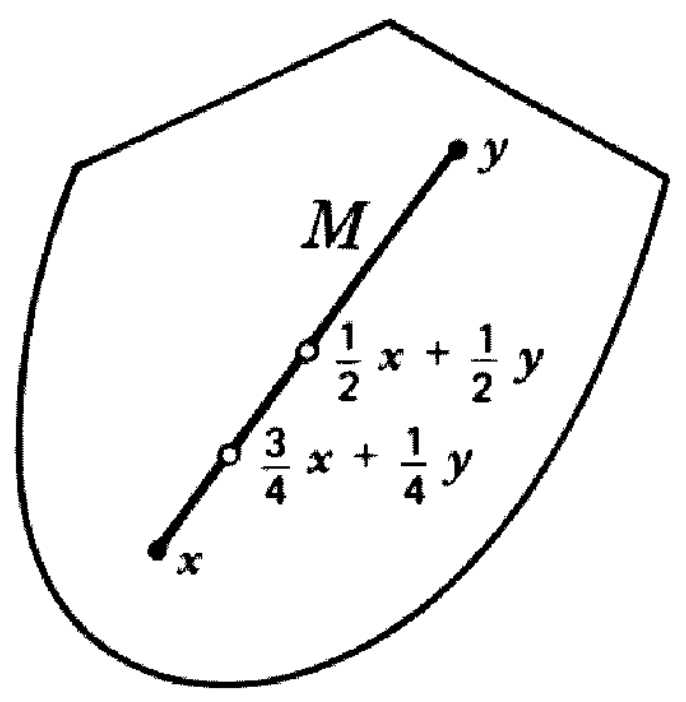
\includegraphics[width=\textwidth]{kreyszig/assets/sec2-2-ex11-a.png}
         \caption{Convex.}
         \label{fig:sec2-2-ex11-a}
     \end{subfigure}
     \hfill
     \begin{subfigure}[b]{0.45\textwidth}
         \centering
         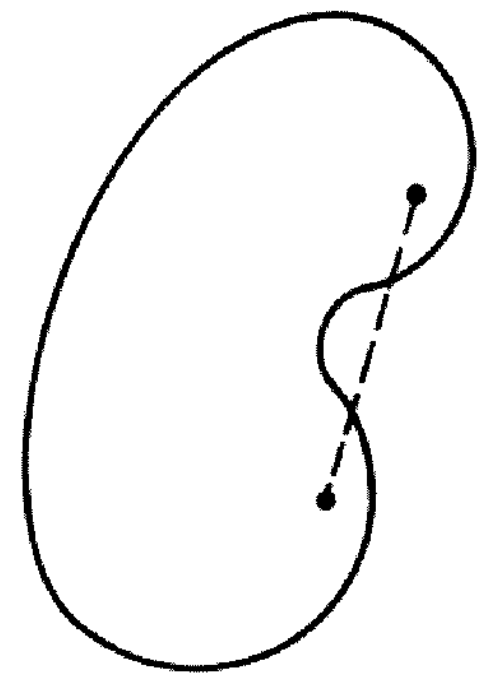
\includegraphics[width=\textwidth]{kreyszig/assets/sec2-2-ex11-b.png}
         \caption{Not convex.}
         \label{fig:sec2-2-ex11-b}
     \end{subfigure}
     \hfill
    \caption{Illustrative examples of convex and nonconvex sets.}
    \label{fig:sec2-2-ex11}
\end{figure}
\end{exercise}
\begin{proof}
Let $x,y\in\bar{B}(0;1)$, then $\norm{x}\leq 1$ and $\norm{y}\leq 1$. Furthermore, let $0\leq\alpha\leq 1$. We have $\norm{\alpha x+(1-\alpha)y} =\norm{\alpha x}+\norm{(1-\alpha)y} =\absoluteValue{\alpha}\norm{x}+\absoluteValue{(1-\alpha)}\norm{y}\leq \alpha+(1-\alpha)=1$, so that $\alpha x+(1-\alpha)y\in\bar{B}(0;1)$, as required.
\end{proof}

\begin{exercise}{12}
Using exercise 11, show that $\phi(x)=(\sqrt{\absoluteValue{x_1}}+\sqrt{\absoluteValue{x_2}})^2$ does not define a norm on the vector space of all ordered pairs $x=(x_1,x_2)$, of real numbers. Sketch the curve $\phi(x)=1$ and compare it with \Cref{fig:sec2-2-ex12}
\begin{figure}[H]
    \centering
    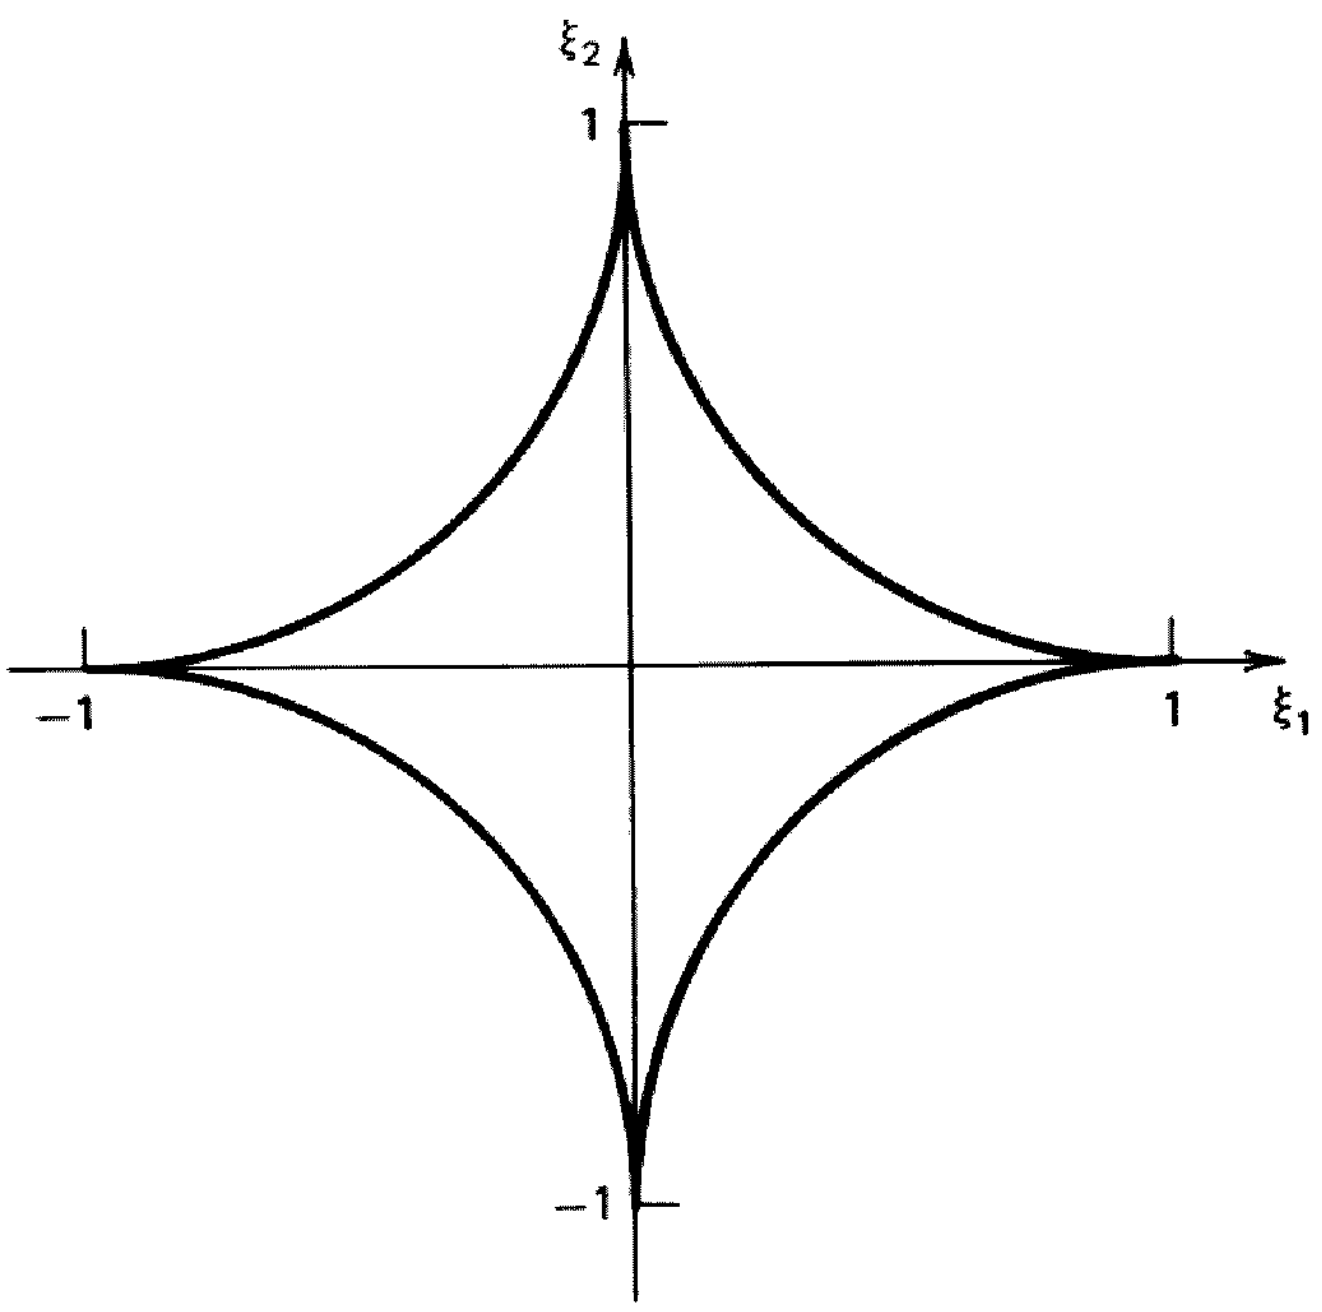
\includegraphics[width=0.5\textwidth]{kreyszig/assets/sec2-2-ex-12.png}
    \caption{Curve $\phi(x)=1$}
    \label{fig:sec2-2-ex12}
\end{figure}
\end{exercise}
\begin{proof}
Let $x=(1,0)$ and $y=(0,1)$, then $\norm{x}=\norm{y}=1$, so that $x,y\in\bar{B}(0;1)$. Let $\alpha=0.5$. We have $\phi(\alpha x+(1-\alpha)y) =(\sqrt{\absoluteValue{0.5}}+\sqrt{\absoluteValue{0.5}})^2 =(2\sqrt{1/2})^2 =\sqrt{4/2}^2 =\sqrt{2}^2 =2$, so that $\bar{B}(0;1)$ is not convex and $\phi(x)$ is not a norm.
\end{proof}

\begin{exercise}{13}
Show that the discrete metric on vector space $X\neq\set{0}$ cannot be obtained from a norm. (Cf. 1.1-8).
\end{exercise}
\begin{proof}
Let $x,y\in X$ and $\alpha$ not 1 nor 0 be a scalar, so that $x\neq y$ and thus $\alpha x\neq \alpha y$. We have $d(\alpha x,\alpha y)=1=d(x,y)$, so that $d$ is not translation invariant. By the contrapositive of 2.2-9 it must be the case $d$ is not induced by a norm.
\end{proof}

\begin{exercise}{15 (Bounded set)}
Show that a subset $M$ in a normed space $X$ is bounded if and only if there is a positive number $c$ such that $\norm{x}\leq c$ for every $x\in M$. (For the definition see exercise 6 in 1.2).
\end{exercise}
\begin{proof}
($\Rightarrow$) Suppose $M$ is bounded. Let $\sup_{x,y\in A}d(x,y)=c$, where $c<\infty$. Fix $y\in M$. From exercise 3, we have that for all $x\in M$, $\norm{x}\leq \norm{x-y}+\norm{y} <c+\norm{y}$. Since $y$ is fixed, we can define $c'=c+\norm{y}$ so that for all $x\in M$, it holds that $\norm{x}<c'$.

($\Leftarrow$) Suppose there exists a positive number $c$ such that $\norm{x}\leq c$ for all $x\in M$. For any $x,y\in M$ we have $d(x,y)=\norm{x-y} \leq\norm{x}+\absoluteValue{-1}\norm{y}\leq 2c$, thus $\sup_{x,y\in M}d(x,y)<2c$ and $M$ is bounded.
\end{proof}
